\documentclass[journal,10pt,twocolumn]{article}
\usepackage[margin=0.5in]{geometry}
\usepackage[cmex10]{amsmath}
\usepackage{array}
\usepackage{booktabs}
% The preceding line is only needed to identify funding in the first footnote. If that is unneeded, please comment it out.
\usepackage{cite}
\usepackage{amsmath,amssymb,amsfonts}
\usepackage{graphicx}
\usepackage{textcomp}
\usepackage{xcolor}
\usepackage{graphicx}
\graphicspath{{./fig}}{}
\def\BibTeX{{\rm B\kern-.05em{\sc i\kern-.025em b}\kern-.08em
    T\kern-.1667em\lower.7ex\hbox{E}\kern-.125emX}}
\usepackage{tikz}
\usetikzlibrary{shapes.geometric}
\usetikzlibrary{shapes.geometric,angles,quotes}
\begin{document}
\newtheorem{theorem}{Theorem}[section]
\newtheorem{problem}{Problem}
\newtheorem{proposition}{Proposition}[section]
\newtheorem{lemma}{Lemma}[section]
\newtheorem{corollary}[theorem]{Corollary}
\newtheorem{example}{Example}[section]
\newtheorem{definition}[problem]{Definition}
%\newtheorem{thm}{Theorem}[section] 
%\newtheorem{defn}[thm]{Definition}
%\newtheorem{algorithm}{Algorithm}[section]
%\newtheorem{cor}{Corollary}
\newcommand{\BEQA}{\begin{eqnarray}}
\newcommand{\EEQA}{\end{eqnarray}}
\newcommand{\define}{\stackrel{\triangle}{=}}
\newcommand*\circled[1]{\tikz[baseline=(char.base)]{
    \node[shape=circle,draw,inner sep=2pt] (char) {#1};}}
\bibliographystyle{article}
%\bibliographystyle{ieeetr}
\providecommand{\mbf}{\mathbf}
\providecommand{\pr}[1]{\ensuremath{\Pr\left(#1\right)}}
\providecommand{\re}[1]{\ensuremath{\text{Re}\left(#1\right)}}
\providecommand{\im}[1]{\ensuremath{\text{Im}\left(#1\right)}}
\providecommand{\qfunc}[1]{\ensuremath{Q\left(#1\right)}}
\providecommand{\sbrak}[1]{\ensuremath{{}\left[#1\right]}}
\providecommand{\lsbrak}[1]{\ensuremath{{}\left[#1\right.}}
\providecommand{\rsbrak}[1]{\ensuremath{{}\left.#1\right]}}
\providecommand{\brak}[1]{\ensuremath{\left(#1\right)}}
\providecommand{\lbrak}[1]{\ensuremath{\left(#1\right.}}
\providecommand{\rbrak}[1]{\ensuremath{\left.#1\right)}}
\providecommand{\cbrak}[1]{\ensuremath{\left\{#1\right\}}}
\providecommand{\lcbrak}[1]{\ensuremath{\left\{#1\right.}}
\providecommand{\rcbrak}[1]{\ensuremath{\left.#1\right\}}}
\newcommand{\sgn}{\mathop{\mathrm{sgn}}}
%\providecommand{\hilbert}{\overset{\mathcal{H}}{ \rightleftharpoons}}
\providecommand{\system}{\overset{\mathcal{H}}{ \longleftrightarrow}}
	%\newcommand{\solution}[2]{\textbf{Solution:}{#1}}
\newcommand{\solution}{\noindent \textbf{Solution: }}
\newcommand{\cosec}{\,\text{cosec}\,}
\providecommand{\dec}[2]{\ensuremath{\overset{#1}{\underset{#2}{\gtrless}}}}
\newcommand{\myvec}[1]{\ensuremath{\begin{pmatrix}#1\end{pmatrix}}}
\newcommand{\mydet}[1]{\ensuremath{\begin{vmatrix}#1\end{vmatrix}}}
	\newcommand*{\permcomb}[4][0mu]{{{}^{#3}\mkern#1#2_{#4}}}
\newcommand*{\perm}[1][-3mu]{\permcomb[#1]{P}}
\newcommand*{\comb}[1][-1mu]{\permcomb[#1]{C}}
%\numberwithin{equation}{section}
\numberwithin{equation}{subsection}
%\numberwithin{problem}{section}
%\numberwithin{definition}{section}
\let\vec\mathbf
\title{
{Finding the maximum profit by optimizing the Machines with certain parameters\\
Using basic Optimization}\\

\thanks {Meer Tabres Ali as an intern with FWC IIT Hyderabad. *The author is with the Department of Electrical Engineering, Indian Institute of Technology, Hyderabad 502285 India e-mail: gadepall@iith.ac.in. All content in this manual is released under GNU GPL. Free and open source.}
}
\author{Meer Tabres Ali and G V V Sharma}
\maketitle
\tableofcontents
\section{Problem statement}
A manufacturer produces nuts and bolts. It takes 1 hour of work on machine A
and 3 hours on machine B to produce a package of nuts. It takes 3 hours on
machine A and 1 hour on machine B to produce a package of bolts. He earns a
profit of Rs17.50 per package on nuts and Rs 7.00 per package on bolts.\\
How many packages of each should be produced each day so as to maximise his
profit, if he operates his machines for at the most 12 hours a day?.
\section{Considerations}

\vspace{0.2cm}
\begin{flushleft}
As per given data, the following table has been prepared.\\
\end{flushleft}
\vspace{0.3cm}
\begin{table}[htbp]
    \centering
\setlength\extrarowheight{2pt}
\begin{tabular}{|c|c|c|c|c|c|} \hline
&  &\textbf{Machine}&\textbf{Machine}& \\
	\textbf{Symbol} & \textbf{Name} &\textbf{A}&\textbf{B}&\textbf{Profit}\\
	\hline
	$\vec{x}$ & nuts & 1x&3x & 17.5x\\  \hline
	$\vec{y}$ & bolts & 3y&1y & 7y\\ \hline
	$\vec{Sum}$ & x+y & x+3y& 3x+y & 17.5x+7y\\ \hline
	$\vec{t}$ & time & 12 h & 12 h & \\ \hline

\end{tabular}
\caption{\label{tab:widgets}Considerations}
\end{table}

\section{Plot to optimize machines to get maximum profit}
\vspace{0.25cm}
Plot of the lines, x+3y=12 and 3x+y=12 which are derived from the given data.
\begin{figure}[h]
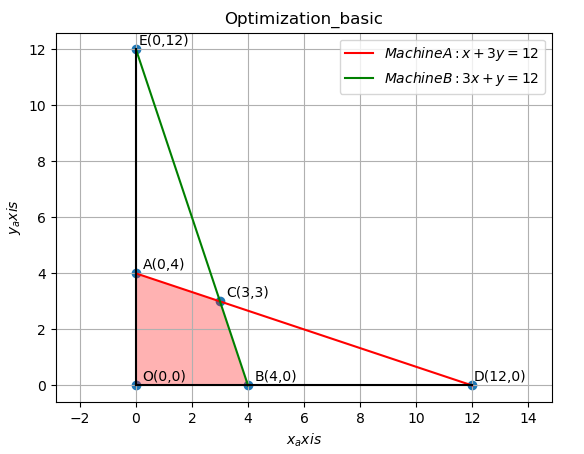
\includegraphics[width=1\columnwidth]{optbasic.png}
\caption{Optimization of Machince A and B}
\label{Optimization of Machince A and B}
\end{figure}

\section{Solution}
\subsection{Deriving constraints from given data}
\begin{flushleft}
Let $\vec{x}$ be the no. of nuts and $\vec{y}$ be the no. of bolts.\\
\end{flushleft}
\vspace{0.25cm}

\begin{flushleft}
We have to maximize $\vec{x}$ and $\vec{y}$ if the factory worked at capacity of 12 hours per day. Then the values of $\vec{x}$ and $\vec{y}$ should be considered as positive, \\
\end{flushleft}
\begin{equation}
x\ge 0,   y\ge 0
\end{equation}

\begin{flushleft}
As per the given data, to produce $\vec{x}$ number nuts, Machine $\vec{A}$ takes 1 hour and Machine $\vec{B}$ takes 3 hours.\\
And, to produce $\vec{y}$ number bolts, Machine $\vec{A}$ takes 3 hours and Machine $\vec{B}$ takes 1 hour.\\
\end{flushleft}
\begin{flushleft}
Since we have only 12 hours of machine working time, we will use the following constraints:\\
\vspace{0.2cm}
For Machine \textbf{A:}
\end{flushleft}
\begin{equation}
x+3y \le 12
\end{equation}
\begin{flushleft}
For Machine \textbf{B:}
\end{flushleft}
\begin{equation}
3x+y \le 12  
\end{equation}
\begin{flushleft}
The above equations can be expressed in vector form as,
\end{flushleft}
\vspace{0.15cm}
\begin{equation}
    \myvec{1 & 3 \\ 3 & 1} \vec{x} \preceq \myvec{12\\12}
\end{equation}

\begin{flushleft}
Let z is the maximum profit, from the table1, z can be expressed as,
\end{flushleft}
\begin{equation}
17.5x+7y=z
\end{equation}

\begin{flushleft}
The optimization is done by using cvxpy packages using python language, and the Maximum profit has been found equal to Rs. 73.50\\
\vspace{0.25cm}
By solving the above inequalities in python using cvxpy packages the value of $\vec{x}$ is :
\begin{equation}
    \vec{x} = \myvec{3\\3}
\end{equation}
Therefore, 3 packages of nuts and 3 packages of bolts should be produced each day to get the maximum profit Rs. 73.50
\end{flushleft}


\begin{flushleft}
\subsection{Finding points of intersections on x and y-axes by line x+3y=12}
It is given that, the profit due to nuts is Rs.17.5 and due to bolts is Rs. 7 .
\end{flushleft}
The points of intersection on y and x-axes by line x+3y$\le$ 12 are\\
\center
$\vec{A} =\myvec{0\\4}$  and $\vec{D} =\myvec{12\\0}$ \\
\endcenter
\begin{flushleft}
\subsection{Finding points of intersection on x and y-axes by line 3x+y=12}
\end{flushleft}

The points of intersection on x and y-axes by line 3x+y$\le$ 12 are\\
\center
$\vec{B} =\myvec{4\\0}$  and $\vec{E} =\myvec{0\\12}$ \\
\endcenter
\begin{flushleft}
\subsection{Finding point of intersection of lines x+3y=12 and 3x+y=12}
\end{flushleft}
On solving the lines x+3y$\le$ 12 and 3x+y$\le$ 12, their point of intersection can be expressed as,
\center
$ \vec{C}=\myvec{3\\3}$
\endcenter
\begin{flushleft}
Therefore, the corner points of the feasible region intersected by above two lines are O(0, 0), A(0, 4), B(4, 0) and C(3, 3) as shown in figure.
\end{flushleft}
\begin{flushleft}
\subsection{Finding maximum profit from the graph with points}
Let z is the maximum profit, the z can be expressed as,
\end{flushleft}
\begin{equation}
17.5x+7y=z
\end{equation}
\begin{flushleft}
The values of Z at these points are as follows:\\
\end{flushleft}
\vspace{0.25cm}

\setlength\extrarowheight{2pt}
\begin{table}
\begin{tabular}{|c|c|c|} \hline
	\textbf{Corner Point} & \textbf{z=17.5x+7y} &\textbf{Remarks}\\
	\hline
	O=$\myvec{0\\0}$ & 0 & \\  \hline
	A=$\myvec{0\\4}$ & 28 & \\ \hline
	C=$\myvec{3\\3}$ & 73.5 & Maximum\\ \hline
	B=$\myvec{4\\0}$ & 70 &  \\ \hline
\end{tabular}
\caption{\label{tab:widgets}Values of $\vec{z}$ }
\end{table}

\begin{flushleft}
From the table, the maximum value of z is Rs. 73.50 is found at the corner point C(3, 3).\\
\vspace{0.25cm}
Therefore, 3 packages of nuts and 3 packages of bolts should be produced each day to get the maximum profit Rs. 73.50
\end{flushleft}
\section{Software}
\centering
Download the codes given in the link below and execute them.\\
\begin{table}[h]
\centering
\begin{tabular}{|c|} \hline
\rule{0pt}{10pt} 
https://github.com/meertabresali-FWC-IITH/project/blob \\
/main/Asgn7.opt.basic/optbasic.py\\
\\\hline
 \end{tabular}
\end{table}
\section{Conclusion}
\begin{flushleft}
1. From the table, the maximum value of z is Rs. 73.50 and it is found at the corner point C(3, 3).\\
\vspace{0.25cm}
2. Therefore, 3 packages of nuts and 3 packages of bolts should be produced each day to get the maximum profit Rs. 73.50
\end{flushleft}



\end{document}
